% INTRODUCTION
%
% !TEX root = ../thesis-main.tex
%
%\part{Introduction}
\chapter{Introduction}
\label{chap:intro}

%\cleanchapterquote{You can’t do better design with a computer, but you can speed up your work enormously.}{Wim Crouwel}{(Graphic designer and typographer)}

Introductory paragraph(s) here

\section{Context: The IFCASL project}
\label{sec:intro:ifcasl}

The work reported here has been conducted in the context of the ongoing research project ``Individualized Feedback in Computer-Assisted Spoken Language Learning (IFCASL)'' at the University of Saarland (Saarbrücken, Germany) and LORIA (Nancy, France). 
%TODO more info
%TODO can I cite project proposal?

The ultimate goal of the project is to take initial steps toward the development of a CAPT system targeting, on the one hand, native (L1) French speakers learning German as a foreign language (L2), and on the other, L1 German speakers learning French as their L2. To this end, a bidirectional learner speech corpus has been recorded, comprising phonetically diverse utterances in French and German spoken by both native speakers and non-native speakers with the other language as L1 \citep{Fauth2014,Trouvain2013}.  

This thesis will focus exclusively on French L1 speakers learning German as L2. The German-language subset of the IFCASL corpus will be instrumental in training and testing the automatic diagnosis and feedback systems which this work aims to develop. Futhermore, those systems will be designed with a view to contributing to the overall set of software developed in the context of the IFCASL project, such that they will be as compatible as possible with the other tools developed and used by the IFCASL team. %TODO reword that


\section{Objectives}
\label{sec:intro:objectives}

The main objective of this work is to investigate the automatic treatment of lexical stress errors in the context of a CAPT system for French learners of German. This includes, on the one hand, an examination of the ways in which lexical stress errors of the type made by French L1 speakers when speaking German as L2 can be reliably detected and measured %TODO reword
automatically, and on the other, an exploration of the types of multimodal feedback on such errors that can be automatically delivered based on the aforementioned error detection. 
The intented outcome of these investigations is a prototype CAPT tool, illustrated in \ref{fig:hourglass}, which can diagnose lexical stress errors in different ways and present learners with different types of feedback on these errors, such that researchers can use this modular system to study the impact of various assessment and feedback types on learner outcomes, user engagement, and other factors impacting the success of a CAPT system. 

		\begin{figure}[htb]
			\centering
			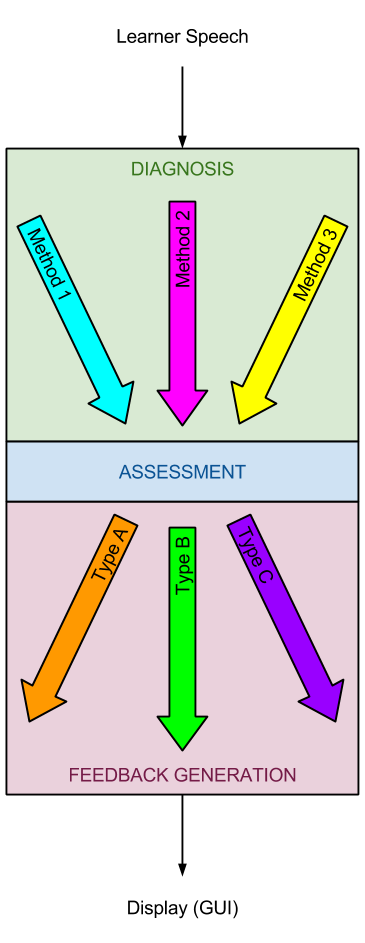
\includegraphics[width=.3\textwidth]{../img/hourglass}
			\caption{Conceptual diagram of the prototype CAPT tool.}
			\label{fig:hourglass}
		\end{figure}

Once more is known about which diagnosis/feedback types should be delivered to which learners in which situations, this tool could become a useful component to a fully-fledged CAPT system, in which learner models and other intelligent components automatically decide which modules of the tool to activate. %TODO figure(s)

\section{Thesis overview}
\label{sec:intro:overview}

{\thesisparagraphfont Chapter 2} introduces Computer-Assisted Pronunciation Training in the context of pronunciation teaching in foreign-language education and computer-based and intelligent tutoring systems, and outlines the phonetic and phonological differences between French and German as well as the motivation for focusing on lexical stress errors in this work.

%TODO flesh out
%TODO future or present tense?

{\thesisparagraphfont Chapter 3} will introduce the systems that have been developed, and the technology used to build them.

{\thesisparagraphfont Chapter 4} will detail the system for assessing learner speech in terms of lexical stress errors.

{\thesisparagraphfont Chapter 5} will describe the multimodal feedback options that the system can deliver.

{\thesisparagraphfont Chapter 6} will summarize the contributions of this work and outlines some interesting future directions to build on these contributions.



